\chapter{Forecasts for Orbit Monitoring}
\label{ch:xforecast}

The thesis measured the mass and distance of \sgra{} from the orbit of S2 and
bounded the no-hair parameter $\epsq$ with the \citet{Gillessen2017} data.
This chapter asks what continued monitoring of S2 can add, and what could
make it mislead. It uses the thesis' own forward model, the full GR orbit
with Rømer delay and relativistic redshift, on synthetic data. Four questions
are addressed:
\begin{enumerate}
\item how fast the no-hair constraint improves as orbits accumulate;
\item when S2 can reveal frame dragging;
\item how an extended mass around \sgra{} couples to the no-hair parameter;
\item how large a false no-hair signal an extended mass produces if it is
left out of the fit.
\end{enumerate}

\section{Method}

\emph{Truth and data.} The true orbit is the thesis' S2 fit, with the
reference-frame nuisances set to the centres of their priors. Noise-free
synthetic data are made with the forward model at three kinds of epochs.
\begin{itemize}
\item The real \citet{Gillessen2017} epochs and errors: $\XFcGnAst$
astrometric and $\XFcGnRv$ radial-velocity points spread over $\XFcGspan$\,yr.
\item A \emph{GRAVITY-era} continuation from 2017.0, with $\XFcGravRate$
astrometric epochs per year at $\XFcGravAst\,\muas$ per coordinate and
$\XFcGravRvRate$ radial velocities per year at $\XFcGravRv$\,km\,s$^{-1}$.
These are the precision and cadence GRAVITY reports for 2016.7--2019.7: 54
interferometric positions with rms uncertainty $\approx 65\,\muas$, and
spectra with $\approx 12$\,km\,s$^{-1}$ uncertainty taken 3--6 times a year
\citep{Gravity2020}.
\item An \emph{existing-quality} continuation that repeats the
adaptive-optics-era sampling of the \citet{Gillessen2017} data: $\XFcExRate$
positions per year at $\XFcExAst$\,mas, and $\XFcExRvRate$ radial
velocities per year at $\XFcExRv$\,km\,s$^{-1}$ (medians of those data).
\end{itemize}
Sampling is uniform in time, with no seasonal gaps, confusion or frame
systematics, so the forecasts below are idealised.

\emph{Forecasts and biases.} Forecast uncertainties come from the Fisher
matrix, $F = J^{\rm T} W J$ plus the thesis' frame priors. Here $J$ is the
central-difference Jacobian of the forward model with respect to its 13 orbit
and frame parameters, plus whichever of $\epsq$, $\astar$ and the extended
mass are free, and $W$ holds the inverse data variances.

The finite-difference steps need care. Around a pericentre passage S2 moves
fastest, along a sharply curved path, so anything
that shifts the time of passage (the mass, distance, semi-major axis or
$\epsq$) changes the predicted positions non-linearly. With the thesis' steps,
which were tuned for its imaging-era data, the Fisher matrix for the
GRAVITY-era data sets therefore depended on the steps. Here those steps are
four to eight times smaller. Halving or doubling any of them, together or one
at a time, now moves no forecast quoted in this chapter by more than
$\XFcStepCheck$ per cent.

Three further checks support the method. On the \citet{Gillessen2017} epochs,
the Fisher matrix gives $\sigma(\epsq) = \XFcSigEpsFisher$, against
$\XFcSigEpsThesis$ from the thesis' profile-likelihood fit to the real data
($\XFcSigEpsDiff$ per cent apart), and $\sigma(M)$ agrees to $\XFcSigMDiff$
per cent. For the GRAVITY-era data sets, the Fisher $\sigma(\epsq)$ agrees
with the curvature of full profile-likelihood fits within $\XFcProfAgree$
per cent (below). Biases, finally, are not linearised at all. An effect that
is present in the data but absent from the model is fitted with the thesis'
own fitter: the 13-parameter Ceres fit for $M$ and $R_0$, and the thesis'
profile likelihood in $\epsq$ (13-parameter fits at fixed $\epsq$). The
profile is not optional. Ceres differentiates numerically with a step of
$10^{-6}$ times the parameter, floored at $\sqrt{\epsilon_{\rm mach}} \approx
1.5\times10^{-8}$. At $\epsq = 0$ that step is many orders of magnitude below
any change the orbit can register, so a direct 14-parameter fit cannot move
$\epsq$ away from its starting value. The thesis' quoted best fit,
$\epsq = 0$, is that starting value. Its interval comes from the profile and
is unaffected.

\emph{The extended mass.} Stars, stellar remnants or dark matter around \sgra{}
would add a spherical mass distribution. We model it, as \citet{Gravity2020}
did, as a \citet{Plummer1911} sphere with scale radius $\XFcPlummer''$. It
enters the metric through its Newtonian potential in $g_{tt}$; its own
post-Newtonian terms are smaller by a further $O(M/r)$. Two unit tests guard
the implementation. Switched off, the model is bit-identical to the thesis
model. And a sphere ten times wider than the orbit reproduces, to within
3 per cent, the textbook retrograde precession of a homogeneous core,
$\Delta\omega = -3\pi f (a/b)^3\sqrt{1-e^2}$ per orbit. As in
\citet{Gravity2022}, its size is quoted as the fraction of $M$ enclosed
within S2's apocentre ($\XFcApo''$), which holds $\XFcEncl$ per cent of the
sphere's mass.

\section{The no-hair reach grows faster than $1/\sqrt{N}$}

The thesis extrapolated its no-hair bound by scaling the uncertainty as
$1/\sqrt{N}$ with the number of orbits. Ten further orbits of existing quality
would then shrink $\sigma(\epsq)$ by a factor $\XFcTenGainThesis$, to
$\XFcTenThesis$. The Fisher forecast for exactly that data set gives
$\sigma(\epsq) = \XFcTenFisher$, a gain of $\XFcTenGain$
(Fig.~\ref{fig:xforecast}, left).

The difference is structural. $\epsq$ acts on S2 almost only through a
\emph{secular} precession of its pericentre, and the \citet{Gillessen2017}
data contain a single pericentre passage (2002). Within one orbit, the
orientation elements absorb most of the quadrupole's effect. Each further
passage measures the accumulated advance directly, and a drift measured over a
baseline $T$ improves as $T^{-3/2}$, not $T^{-1/2}$. The jumps in the
existing-quality curve sit at the pericentre passages. The $1/\sqrt{N}$
figure in the thesis is therefore a strong underestimate of what monitoring
can achieve.

GRAVITY-era astrometry ($\XFcGravAst\,\muas$ per coordinate at $\XFcGravRate$
epochs per year, against $\XFcExAst$\,mas at $\XFcExRate$ for the
adaptive-optics data) gains faster still: $\sigma(\epsq)$ falls to
$\XFcEpsGravEight$ after 8 years, $\XFcEpsGravSixteen$ after 16 (one orbit),
$\XFcEpsGravThirtyTwo$ after 32 and $\XFcEpsGravSixtyFour$ after 64. That is
two orders of magnitude within a few decades. It is still far from the Kerr
quadrupole itself, $|\tilde q| = \astar^2 < 1$ in units of $M^3$, so S2 is
too far out to test the no-hair theorem at that level, as the thesis argued.

\begin{figure}
\centering
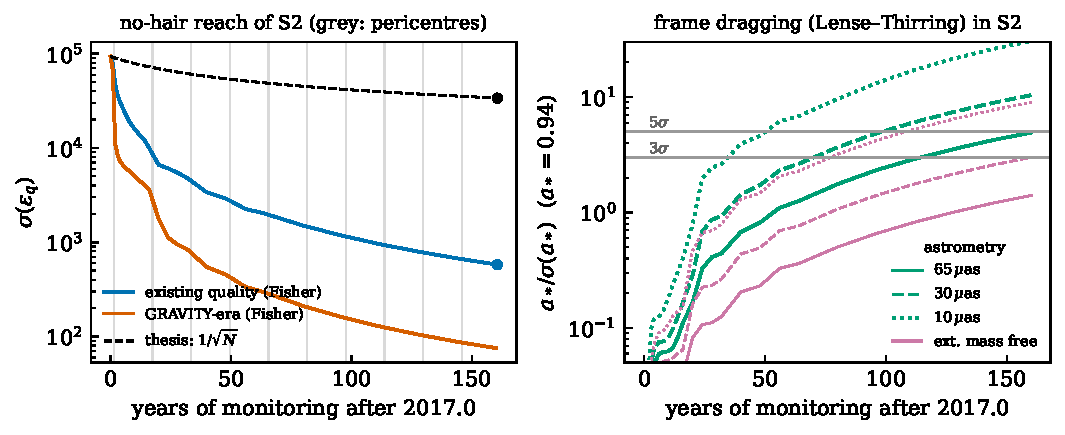
\includegraphics[width=\textwidth]{figures/fig_x_forecast.pdf}
\caption{Left: forecast uncertainty of the no-hair parameter versus
monitoring time after 2017.0, for the two continuations of the data (grey
lines: S2's pericentre passages). The dashed curve is the thesis' $1/\sqrt{N}$
extrapolation; the dots compare it with the Fisher forecast at ten more
orbits. Right: significance of the spin of \sgra{} ($\astar = 0.94$,
Lense--Thirring and Kerr quadrupole) for three astrometric precisions per
coordinate (green; purple: with an extended mass fitted at the same time).
Spin axis along the line of sight.}
\label{fig:xforecast}
\end{figure}

\section{Frame dragging}

At $\astar = 0.94$, frame dragging shifts S2's pericentre by only
$\PrecLT$~arcmin per orbit, against $\PrecSchw$~arcmin for the Schwarzschild
advance (both from the thesis' S2 fit). GRAVITY measured the Schwarzschild
advance with a 19 per cent uncertainty \citep{Gravity2020}. With $\astar$
free in the Kerr model
(Fig.~\ref{fig:xforecast}, right), the spin reaches $3\sigma$ after
$\XFcLtThreeSixtyFive$\,yr of monitoring at $65\,\muas$, and $5\sigma$ after
$\XFcLtFiveSixtyFive$\,yr. Better astrometry helps strongly: at $30\,\muas$
the times are $\XFcLtThreeThirty$ and $\XFcLtFiveThirty$\,yr, and at
$10\,\muas$ they are $\XFcLtThreeTen$ and $\XFcLtFiveTen$\,yr.

These times assume that nothing else precesses the orbit. If an extended mass
is fitted at the same time, they become $\XFcLtThreeSixtyFiveMarg$ and
$\XFcLtFiveSixtyFiveMarg$\,yr at $65\,\muas$, $\XFcLtThreeThirtyMarg$ and
$\XFcLtFiveThirtyMarg$\,yr at $30\,\muas$, and $\XFcLtThreeTenMarg$ and
$\XFcLtFiveTenMarg$\,yr at $10\,\muas$. This is the confusion that
\citet{Merritt2010} identified, and that \citet{Gravity2020} noted for their
own extended-mass limit. The direction of the spin axis matters: here it lies
along the line of sight, as throughout the thesis.

\section{The extended mass and the no-hair parameter}

An extended mass and a positive $\epsq$ both advance S2's pericentre
retrogradely, so the two parameters trade against each other. With both free,
their correlation is $\XFcCorrGs$ on the \citet{Gillessen2017} data, and
$\XFcCorrEight$, $\XFcCorrSixteen$ and $\XFcCorrThirtyTwo$ after 8, 16 and
32\,yr of GRAVITY-era monitoring. The extended mass itself is constrained to
$\sigma = \XFcSigEncGs$ per cent of $M$ within the apocentre by the
\citet{Gillessen2017} data alone, and to $\XFcSigEncEight$ per cent after
8\,yr of GRAVITY-era data. The second figure is consistent with the $\approx
0.1$ per cent that GRAVITY achieved with three years of such data
\citep{Gravity2020, Gravity2022}. Fitting the extended mass jointly costs
little: it widens $\sigma(\epsq)$ by factors of only $\XFcInflEight$,
$\XFcInflSixteen$ and $\XFcInflThirtyTwo$ at 8, 16 and 32\,yr
(Fig.~\ref{fig:xdegeneracy}, left).

\emph{Leaving it out} is a different matter (Table~\ref{tab:xbias},
Fig.~\ref{fig:xdegeneracy}, right). Take an extended mass at GRAVITY's present
$1\sigma$ bound, 0.1 per cent of $M$ within the apocentre, fitted with the
pure Kerr model. It produces a false no-hair signal of $\XFcBiasEpsEight\sigma$
after 8\,yr, $\XFcBiasEpsSixteen\sigma$ after 16\,yr and
$\XFcBiasEpsThirtyTwo\sigma$ after 32\,yr; half that mass still gives
$\XFcBiasEpsHalfThirtyTwo\sigma$ at 32\,yr. Here $\sigma$ is the uncertainty
the biased fit itself would quote, from the curvature of its profile. The
mass is biased only slightly, by $\XFcBiasMEight\sigma$,
$\XFcBiasMSixteen\sigma$ and $\XFcBiasMThirtyTwo\sigma$.

Nothing in the fit gives the problem away. Measured against the true Kerr
orbit, the extended mass alters the data by $\chi^2 = \XFcChiSignalEight$,
$\XFcChiSignalSixteen$ and $\XFcChiSignalThirtyTwo$, far more than their
errors, but the orbit elements absorb nearly all of it. The $\chi^2$ the Kerr fit leaves over is only $\XFcChiLeftEight$,
$\XFcChiLeftSixteen$ and $\XFcChiLeftThirtyTwo$. Noise alone scatters the
$\chi^2$ of these $N = \XFcNrowsEight$, $\XFcNrowsSixteen$ and
$\XFcNrowsThirtyTwo$ data values by $\sqrt{2N} = \XFcChiScatterEight$,
$\XFcChiScatterSixteen$ and $\XFcChiScatterThirtyTwo$, so the leftover is
lost in it.

That absorption also defeats linearised estimates. It moves the orbit a long
way along its best-measured direction, where the model is no longer linear.
The linear response about the true orbit recovers only
$\XFcBiasLinRatioThirtyTwo$ of the fitted 32-yr $\epsq$ bias, and for some
data sets it gets the mass bias wrong in sign. Every bias quoted here
therefore comes from a full refit.

So any future no-hair test with S2 must fit an extended mass jointly. Doing so
is cheap. Not doing so turns the extended mass, which can be no larger than
the present bound, into the leading systematic error. The thesis named this
risk in its discussion; these numbers quantify it.

\begin{table}
\centering
\caption{An extended mass (Plummer, scale $\XFcPlummer''$) present in the
data but left out of the fit: biases of the 13-parameter Kerr fit in $M$ and
$R_0$ and the $\chi^2$ it leaves, and the false no-hair signal in the thesis'
$\epsq$ profile. Noise-free data on the \citet{Gillessen2017} epochs, plus
the stated years of GRAVITY-era monitoring. For $M$ and $R_0$, $\sigma$ is the
forecast uncertainty of the same data set; for $\epsq$ it is the uncertainty
the biased fit itself would quote, from the curvature of its profile.}
\label{tab:xbias}
\small\setlength{\tabcolsep}{4pt}
% AUTO-GENERATED by scripts/make_numbers_ext.py — do not edit by hand.
\begin{tabular}{rlrrrrr}
\toprule
$M_{\rm ext}$ [\% of $M$] & data & $\Delta M/\sigma$ & $\Delta R_0/\sigma$ & $\Delta\epsilon_q$ & $\Delta\epsilon_q/\sigma$ & $\chi^2_{\rm left}$ \\
\midrule
0.05 & Gillessen 2017 & +0.02 & +0.02 & $2\,550$ & +0.03 & 0.0034 \\
0.05 & +\,8\,yr & +0.16 & +0.18 & $1\,450$ & +0.24 & 0.41 \\
0.05 & +\,16\,yr & +0.20 & +0.22 & $2\,550$ & +0.68 & 1.3 \\
0.05 & +\,32\,yr & +0.14 & +0.25 & $2\,090$ & +2.48 & 18 \\
0.10 & Gillessen 2017 & +0.05 & +0.03 & $6\,830$ & +0.07 & 0.014 \\
0.10 & +\,8\,yr & +0.32 & +0.37 & $2\,880$ & +0.47 & 1.6 \\
0.10 & +\,16\,yr & +0.42 & +0.45 & $5\,120$ & +1.36 & 5.3 \\
0.10 & +\,32\,yr & +0.35 & +0.56 & $4\,180$ & +4.98 & 73 \\
0.20 & Gillessen 2017 & +0.09 & +0.06 & $1.5\times10^{4}$ & +0.17 & 0.055 \\
0.20 & +\,8\,yr & +0.64 & +0.75 & $5\,780$ & +0.94 & 6.4 \\
0.20 & +\,16\,yr & +0.89 & +0.92 & $1.0\times10^{4}$ & +2.78 & 22 \\
0.20 & +\,32\,yr & +0.71 & +1.13 & $8\,360$ & +9.99 & 300 \\
\bottomrule
\end{tabular}

\end{table}

\begin{figure}
\centering
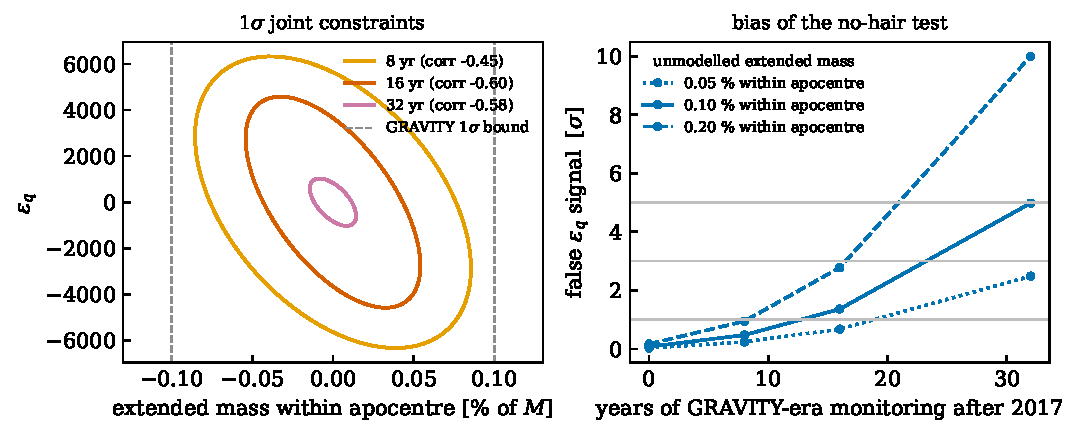
\includegraphics[width=\textwidth]{figures/fig_x_degeneracy.pdf}
\caption{Left: joint $1\sigma$ constraints on the extended mass enclosed
within S2's apocentre and the no-hair parameter, after 8, 16 and 32\,yr of
GRAVITY-era monitoring (grey: GRAVITY's present $1\sigma$ bound). Right: the
false no-hair signal, in units of the forecast $\sigma(\epsq)$, when the
extended mass is left out of the fit.}
\label{fig:xdegeneracy}
\end{figure}
